\section{Results}

We consider the following fiscal policy experiments

\begin{itemize}
	\item Payroll tax cut: Employed individuals benefit from a 2 percentage points lower payroll tax cut. The tax cut is unanticipated and usually lasts for 8 quarters. However, there is a 50\% chance, that the policy is extended by another 8 quarters if the recession is still ongoing in the 8th quarter of the payroll tax cut. 
	\item Unemployment insurance extension: The duration of the unemployment insurance is doubled from 2 to 4 quarters. Agents, that are unemployed when the policy is implemented thus receive up to 4 quarters of unemployment insurance. The policy is unanticipated and active only for one quarter.
	\item Stimulus check: Each individual, independent of employment status, receives an unanticipated payment of \$1200 in one quarter. However, the check is only paid out fully to individuals with a permanent yearly income smaller than 100,000 and not at all to those with a income greater than 150,000. Those within the two thressholds receive a share of the full stimulus check amount proportionate to their position within threshholds.\footnote{For this income group, the check amount is given by $\$1200 (1-\frac{Income-100,000}{50,000})$. For example, an individual with a permanent yearly income of 110,000 receives 80\% of the stimulus, i.e. \$960.}
\end{itemize}

\subsection{Impulse responses}


\begin{figure}
	\centering
	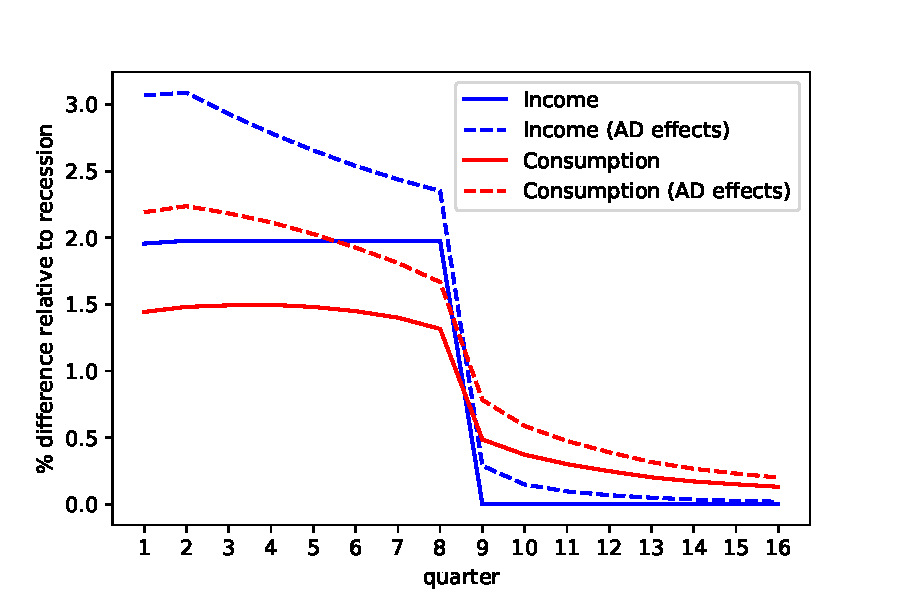
\includegraphics[width=0.8\linewidth]{../Code/HA-Models/FromPandemicCode/Figures/recession_taxcut_relrecession}
	\caption{Impulse responses of aggregate income and consumption to a pay roll tax cut during a recesssion lasting eight quarters with and without aggregate demand effects}
	\label{fig:recessiontaxcutrelrecession}
\end{figure}

\begin{figure}
	\centering
	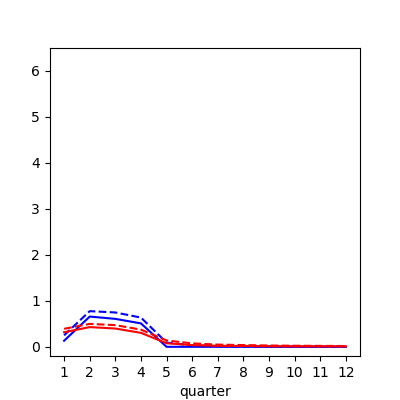
\includegraphics[width=0.8\linewidth]{../Code/HA-Models/FromPandemicCode/Figures/recession_UI_relrecession}
	\caption{Impulse responses of aggregate income and consumption to a UI extension during a recesssion with and without aggregate demand effects}
	\label{fig:recessionuirelrecession}
\end{figure}

\begin{figure}
	\centering
	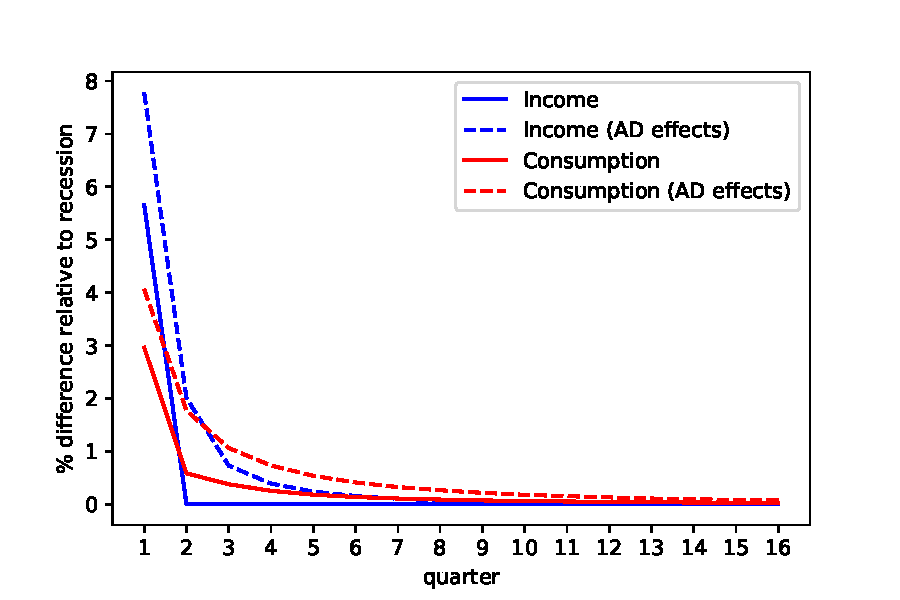
\includegraphics[width=0.8\linewidth]{../Code/HA-Models/FromPandemicCode/Figures/recession_Check_relrecession}
	\caption{Impulse responses of aggregate income and consumption to a stimulus check during a recesssion with and without aggregate demand effects}
	\label{fig:recessioncheckrelrecession}
\end{figure}

\FloatBarrier
\subsection{Multipliers}

Definitions:
\begin{itemize}
	\item The \textit{net present value (NPV)} of a variable X at horizon t is given by
	\begin{equation}
	NPV(t,X) = \sum_{s=0}^{t} \left( \prod_{i=1}^{s} \frac{1}{R_i} \right) X_s
	\end{equation}
	\item The \textit{cummulative multiplier (CM)} of a policy is given by
	\begin{equation}
	CM(t) = \frac{NPV(t,\Delta C)}{NPV (T_{max},\Delta G)}
	\end{equation}
	where $\Delta C$ is the additional aggregate consumption spending in the policy scenario relative to the baseline and $\Delta G$ is the government expenditures caused by the policy.
\end{itemize}

\begin{table} 
	\center
	\input ../Code/HA-Models/FromPandemicCode/Tables/Multiplier.tex
	\caption{Multipliers as well as the share of the policy ocurring during the recession for the three policies considered}
	\label{tab:Multiplier}
\end{table}

\begin{table} 
	\center
	\input ../Code/HA-Models/FromPandemicCode/Tables/Multiplier_RecLengths.tex
	\caption{Multipliers (with AD effects) for different recesssion lengths for the three policies considered}
	\label{tab:Multiplier_RecLengths}
\end{table}

\begin{figure}
	\centering
	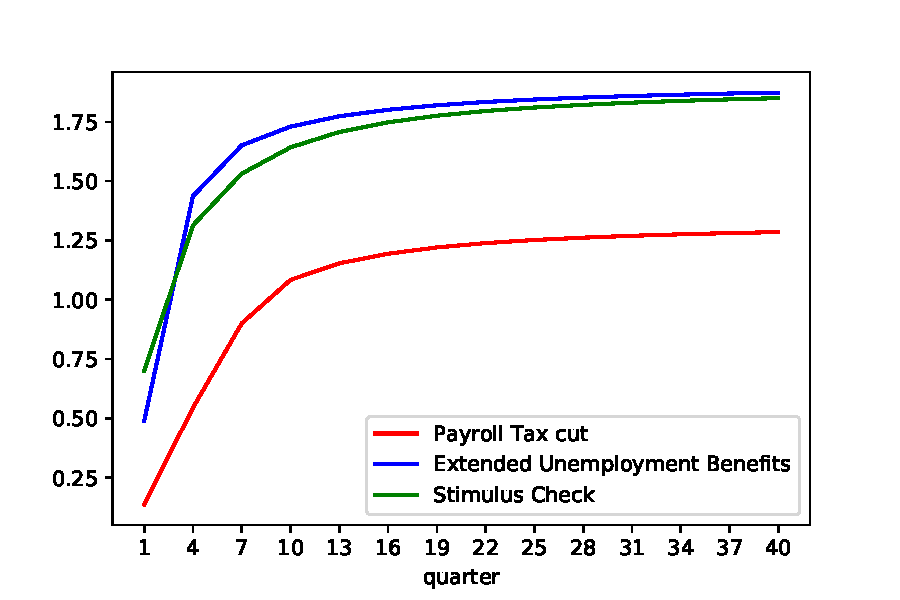
\includegraphics[width=0.8\linewidth]{../Code/HA-Models/FromPandemicCode/Figures/Cummulative_multipliers}
	\caption{Cummulative Multiplier as a function of the horizon in quarters for the three policies considered. Policies are implemented during a recession with AD effects active}
	\label{fig:cummulativemultipliers}
\end{figure}